RRR je struktura podatka za pohranjivanje bit-vektora pomoću koje je moguće u kratkom vremenu izvršiti upite. Navedena struktura je sažeta \engl{Succint data structure}, no unatoč tomu nije ju potrebno u cijelosti raspakirati kako bi se obavio upit nad istom. 

\section{Izgradnja RRR strukture}

Prilikom izgradnje RRR strukture prvi korak je podjela ulaznog niza bitova na blokove, odnosno superblokove. Veličine superbloka i bloka moguće je proizvoljno definirati. Nakon odabira veličine bloka potrebno je izgraditi RRR tablicu.

\begin{figure}[H]
	\centering
	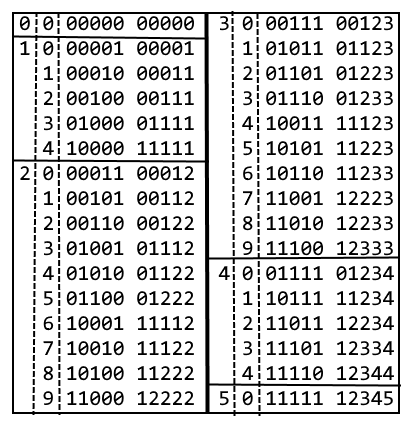
\includegraphics[width = 0.5\textwidth] {img/rrrtable.png}
	\caption{Sadržaj RRR tablice za $b = 5$, preuzeto iz \cite{breberic}}
	\label{fig:rrrtable}
\end{figure}

Tablica je pomoćna struktura koja će se koristiti u izvršavanju upita. Sama tablica će sadržavati sve moguće permutacije blokova za sve moguće rangove za danu veličinu bloka te niz sume rangova do svake pozicije unutar bloka. Implementacijski gledano tablica će sadržavati pokazivače na tablice za svaki rang bloka unutar kojih će biti definirane permutacije tog ranka i odgovarajuća sumu jedinica za svaku poziciju u odgovarajućem bloku. Primjer jedne takve tablice prikazan je na slici \ref{fig:rrrtable}.

Kroz sljedeći primjer bit će prikazana izgradnja RRR strukture iz ulaznog niza bitova, za veličinu bloka $b=5$ i superbloka $f=2$. Na slici \ref{fig:blocks} je prikazana podjelu niza na četiri bloka i dva superbloka. Nakon podjele niza bitova u blokove i superblokove potrebno je za svaki blok odrediti rang te odmak unutar tablice blokova, odnosno pozicija bloka unutar tablice koji odgovara danom bloku. Tako dobiveni parovi se spremaju u niz koji će se koristiti u daljnjim operacijama nad strukturom. Uz navedeni niz, također se sprema i niz parova koji sadrže ukupnu sumu rangova unutar prethodnih superblokova te odmak prvog bloka za pojedini superblok. 

\begin{figure}[H]
	\centering
	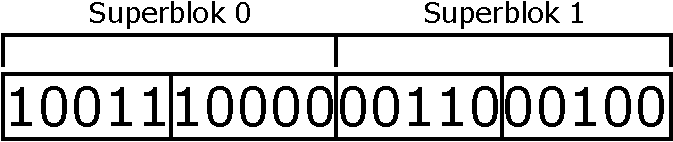
\includegraphics[width=0.6\textwidth]{img/superblocks.pdf}
	\caption{Podjela bit-vektora na blokove i superblokove}
	\label{fig:blocks}
\end{figure} 

Korištenjem tablice \ref{fig:rrrtable} nad primjerom danim na slici \ref{fig:blocks} dobio bi se kodiran niz prikazan u obliku parova $[(3, 4), (1, 4), (2, 2), (1, 2)]$, gdje prvi element para predstavlja rang, a drugi odmak u tablici. Isti taj niz, zapisan kao niz bitova prikazan je na slici \ref{fig:codecseq}. Niz parova suma ranga i odmaka prvog sljedećeg bloka bi ovisio o tome kako se zapisuju navedeni parovi u memoriju. Naime, moguće je navedene parove zapisivati kao dva broja ili ih kodirati tako da se postigne maksimalna memorijska učinkovitost. No takav način kodiranja zahtjeva i dekodiranje prilikom obavljanja upita što može dodatno usporiti brzinu njihova izvršavanja. Razlika u ta dva načina zapisa je u odmaku prvog bloka, za nekodirane nizove odmak je samo indeks prvog slijedećeg bloka, dok za kodirane iznosi broj bitova do odmaka (odmak unutar RRR tablice) prvog slijedećeg bloka. Za primjer dan na slici \ref{fig:blocks} i bez kodiranja taj niz bi iznosio $[(0, 0), (4, 2)]$, dok bi uz kodiranje iznosio $[(0, 3), (4, 16)]$.

\begin{figure}[H]
	\centering
	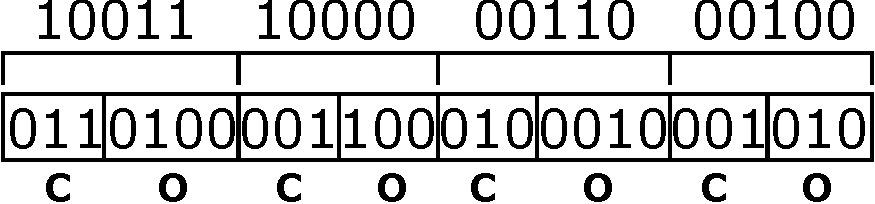
\includegraphics[width=0.6\textwidth]{img/coded.pdf}
	\caption{Ulazni niz \texttt{10011100000011000100} kodiran u RRR strukturu}
	\label{fig:codecseq}
\end{figure}

\subsection{Kodiranje parova}

Kodiranje parova moguće je izvršiti tako da se uzme broj bitova potrebnih za najveći rang bloka unutar RRR tablice odnosno $r\_bit=\lceil(\log_2(b + 1))\rceil$ gdje je $b$ veličina bitova u bloku, dok se broj bita odmaka uzme veličina koja ovisi o rangu $o\_bit=\lceil(\log_2({b \choose r}))\rceil$ gdje je $r$ rang u bloku. Uz pomoć te dvije veličine moguće je jedan par spremiti unutar $o\_bit+r\_bit$ bitova.

\subsection{Dekodiranje parova}

Dekodiranje parova se vrši na način da se prvo dekodira rang jer je broj bitova za kodiranje ranga stalan te je poznat početak bloka. Nakon dekodiranja ranga, iz RRR tablice možemo saznati potreban broj bitova za odmak te dekodirati i sam odmak.

\section{Upiti nad RRR strukturom}

Nad RRR strukturom moguće je obavljati tri vrste upita:

\begin{itemize}
    \item $rank_b(i) $- broj pojavljivanja bita $b$ do pozicije $i$ u ulaznom nizu bitova
    \item $select_b(i)$ - pozicija $i$-tog pojavljivanja bita $b$ u ulaznom nizu bitova
    \item $access(i)$ - bit na $i$-toj poziciji u ulaznom nizu bitova
\end{itemize}

\subsection{\emph{Rank}}

Nad RRR strukturom možemo obavljati \emph{rank1} i \emph{rank0} upite, gdje \emph{rank1} vraća broj bitova postavljenih na $1$ do danog indeksa u nizu, te \emph{rank0} analogno tomu broj bitova postavljenih na $0$. Algoritam \emph{rank1} i \emph{rank0} upita prikazan je pseudokodom \ref{alg:rrr_rank1} i \ref{alg:rrr_rank0}.

\begin{algorithm}[H]
  \floatname{algorithm}{Pseudokod}
  \caption{\emph{rank1} upit nad RRR strukturom, preuzeto iz \cite{bowe-th} i \cite{breberic}}
  \begin{algorithmic}[1]
    \Function{rank1}{$i$}
    \State $i_b \gets \left \lfloor \frac{i}{b} \right \rfloor$
    \State $i_s \gets \left \lfloor \frac{i_b}{b * s} \right \rfloor$
    \State $suma \gets $ rank $i_s$-tog super bloka
    \State $trenutni\_blok \gets $ prvi blok $i_s$ tog super bloka
    \While{$trenutni\_blok \neq i_b$-ti blok}
      \State $suma \gets suma + $ razred od $trenutni\_blok$
      \State $trenutni\_blok \gets $ slijedeći blok
      \State $j \gets i \ \% \ b$
      \State $suma \gets suma + $ pozicija na kojoj se nalazi $j$-ta jedinica u bloku 
      \State{}
      \Return $suma$
    \EndWhile
    \EndFunction
  \end{algorithmic}
  \label{alg:rrr_rank1}
\end{algorithm}

\begin{algorithm}[H]
  \floatname{algorithm}{Pseudokod}
  \caption{\emph{rank0} upit nad RRR strukturom, preuzeto iz \cite{bowe-th} i \cite{breberic}}
  \begin{algorithmic}[1]
    \Function{rank0}{$i$}
      \State{} \Return $i + 1 - $ \Call{rank1}{$i$}
    \EndFunction
  \end{algorithmic}
  \label{alg:rrr_rank0}
\end{algorithm}


\subsection{\emph{Select}}

Kao i za \emph{rank} upite, nad RRR strukturom možemo izvoditi \emph{select1} i \emph{select0} upite. Oni odgovaraju pozicijom $i$-tog bita postavljenog na $1$, odnosno $0$. Algoritam \emph{select1} i \emph{select0} upita prikazan je pseudokodom \ref{alg:rrr_select1} i \ref{alg:rrr_select0}.

\begin{algorithm}[H]
  \floatname{algorithm}{Pseudokod}
  \caption{\emph{select1} upit nad RRR strukturom, preuzeto iz \cite{bowe-th} i \cite{breberic}}
  \begin{algorithmic}[1]
    \Function{select1}{$i$}
    \State $i_s \gets$ indeks superbloka kojem je rank bitova 1 $ < i$
    \State $suma \gets $ rank $i_s$-tog superbloka
    \State $trenutni\_blok$ prvi blok $i_s$-tog superbloka
    \State $indeks \gets i_s * s$
    \While{ima blokova}
      \State $s \gets suma + $ razred od $trenutni\_blok$
      \If{$s \geq i$}
        \State iza\dj{}i iz petlje
      \Else
        \State $suma = s$
      \EndIf
      \State $trenutni\_blok \gets $ sljede\'{c}i blok
      \State $indeks \gets indeks + b$
    \EndWhile
    \State $indeks \gets indeks + $ indeks na kojem se nalazi $(broj-suma)$-ti bit 1 u bloku
    \State{} \Return $indeks$
    \EndFunction
  \end{algorithmic}
  \label{alg:rrr_select1}
\end{algorithm}

\begin{algorithm}[H]
  \floatname{algorithm}{Pseudokod}
  \caption{\emph{select0} upit nad RRR strukturom, preuzeto iz \cite{bowe-th} i \cite{breberic}}
  \begin{algorithmic}[1]
    \Function{select0}{$i$}
    \State $i_s \gets$ indeks super bloka kojem je rank bitova 0 $ < i$
    \State $trenutni\_blok$ prvi blok $i_s$-tog super bloka
    \State $indeks \gets i_s * s$
    \State $suma \gets indeks - $ rank $i_s$-tog super bloka
    \While{ima blokova}
      \State $s \gets suma + (b - $ razred od $trenutni\_blok)$
      \If{$s \geq i$}
        \State iza\dj{}i iz petlje
      \Else
        \State $suma = s$
      \EndIf
      \State $trenutni\_blok \gets $ sljedeći blok
      \State $indeks \gets indeks + b$
    \EndWhile
    \State $indeks \gets indeks + $ indeks na kojem se nalazi $(broj-suma)$-ti bit 0 u bloku
    \State{} \Return $indeks$
    \EndFunction
  \end{algorithmic}
  \label{alg:rrr_select0}
\end{algorithm}

\subsection{\emph{Access}}

\emph{Access} upit vraća vrijednost bita na $i$-toj poziciji. Implementacija se može izvesti pomoću dva poziva \emph{rank1} upita. Algoritam \emph{access} upita prikazan je pseudokodom \ref{alg:rrr_access}.

\begin{algorithm}[H]
  \floatname{algorithm}{Pseudokod}
  \caption{Access operacija nad RRR strukturom \cite{bowe-th}\cite{breberic}}
  \begin{algorithmic}[1]
    \Function{access}{$i$}
      \If{$i = 0$} 
        \State \Return \Call{rank1}{$i$}
      \Else
        \State \Return \Call{rank1}{$i$} - \Call{rank1}{$i - 1$}
      \EndIf
    \EndFunction
  \end{algorithmic}
  \label{alg:rrr_access}
\end{algorithm}
